\noindent
This chapter will describe the steps of the algorithm that we have designed. Each step will be described in detail and with pictures which will help better understand.
\\
For the automatic depth calibration of the camera we must find a set of equivalent points in different images, also known as correspondences. This means that if we identify a point in the image from the Kinect, we must find its equivalent in the image provided by the normal camera. In order to do this, we have created a pattern that we would like to detect. 
\\\\
The pattern that we want to detect is in the shape of a cone with its tip colored green. The color of the tip is not important, the algorithm can be adapted to work with almost any color. For experimental purposes, we have decided to keep the color of tip green. 
\\
An image of the pattern can be seen below:

\begin{center}
	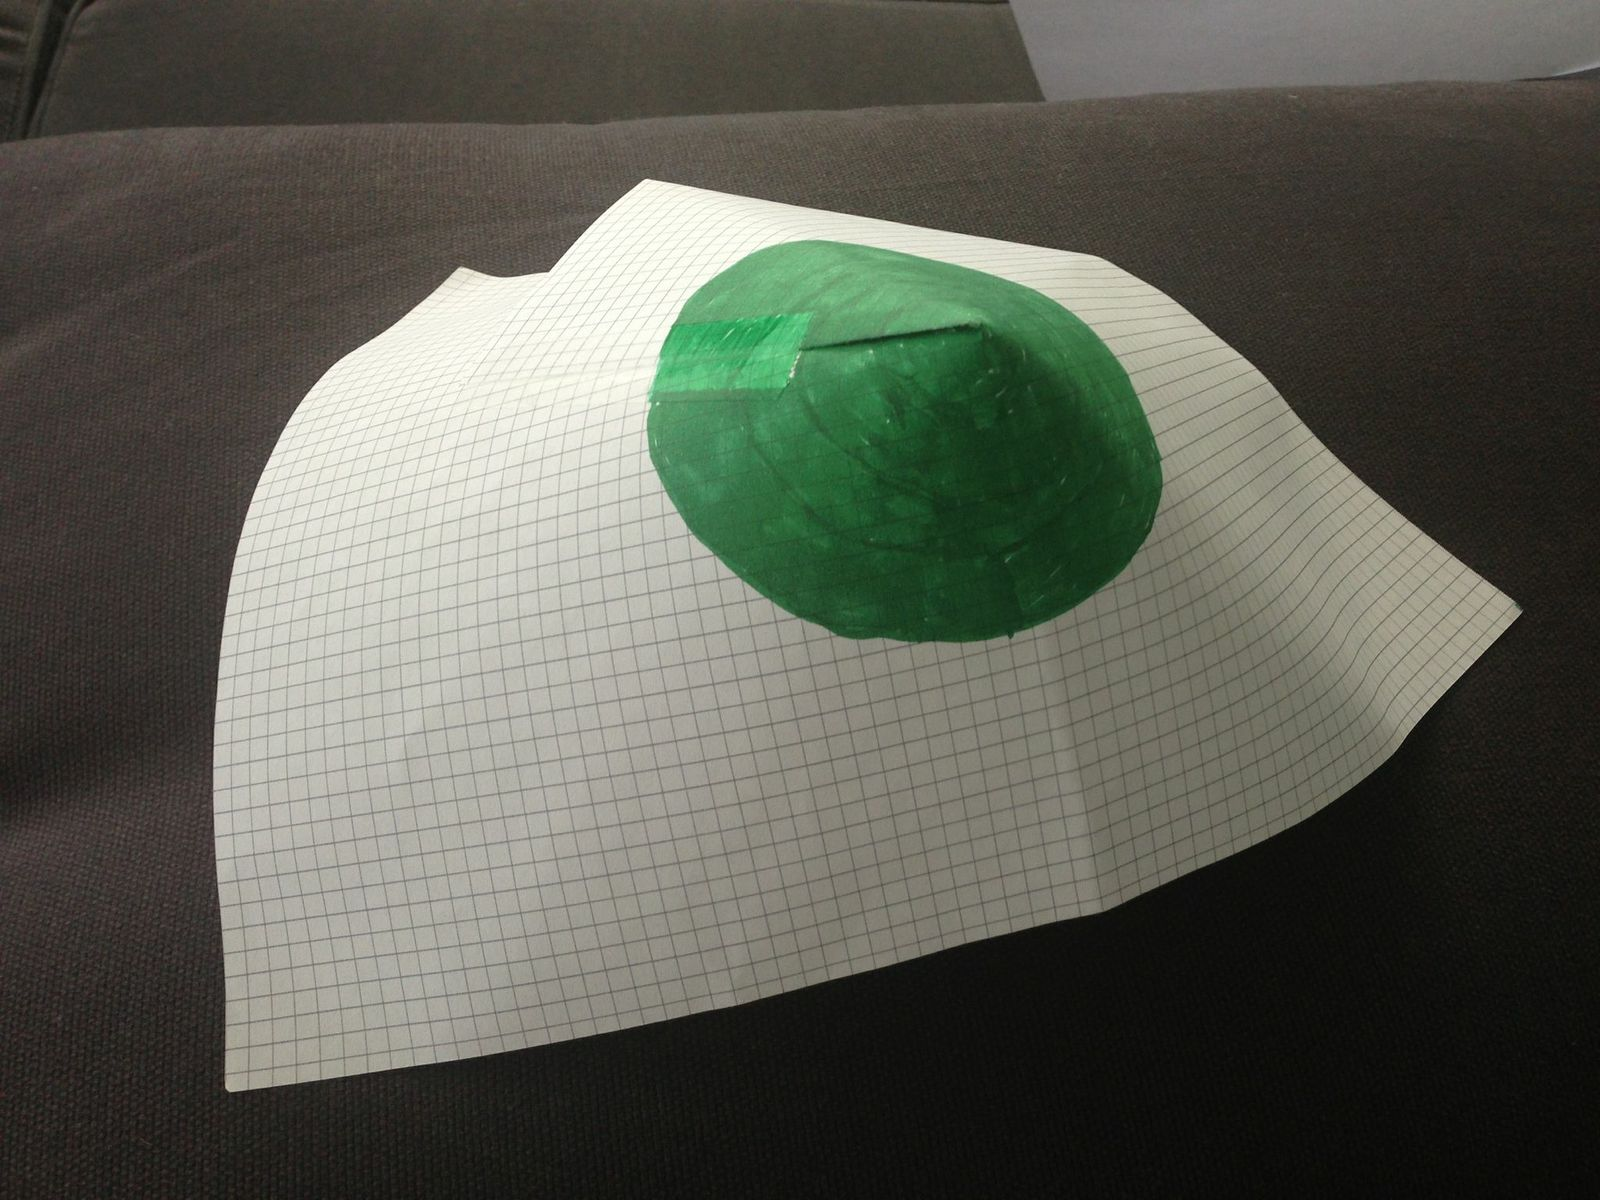
\includegraphics[scale=0.1]{images/pattern_1.jpg}
 	\captionof{figure}{Small pattern}
	\label{fig:small_pattern}
\end{center}

\begin{center}
	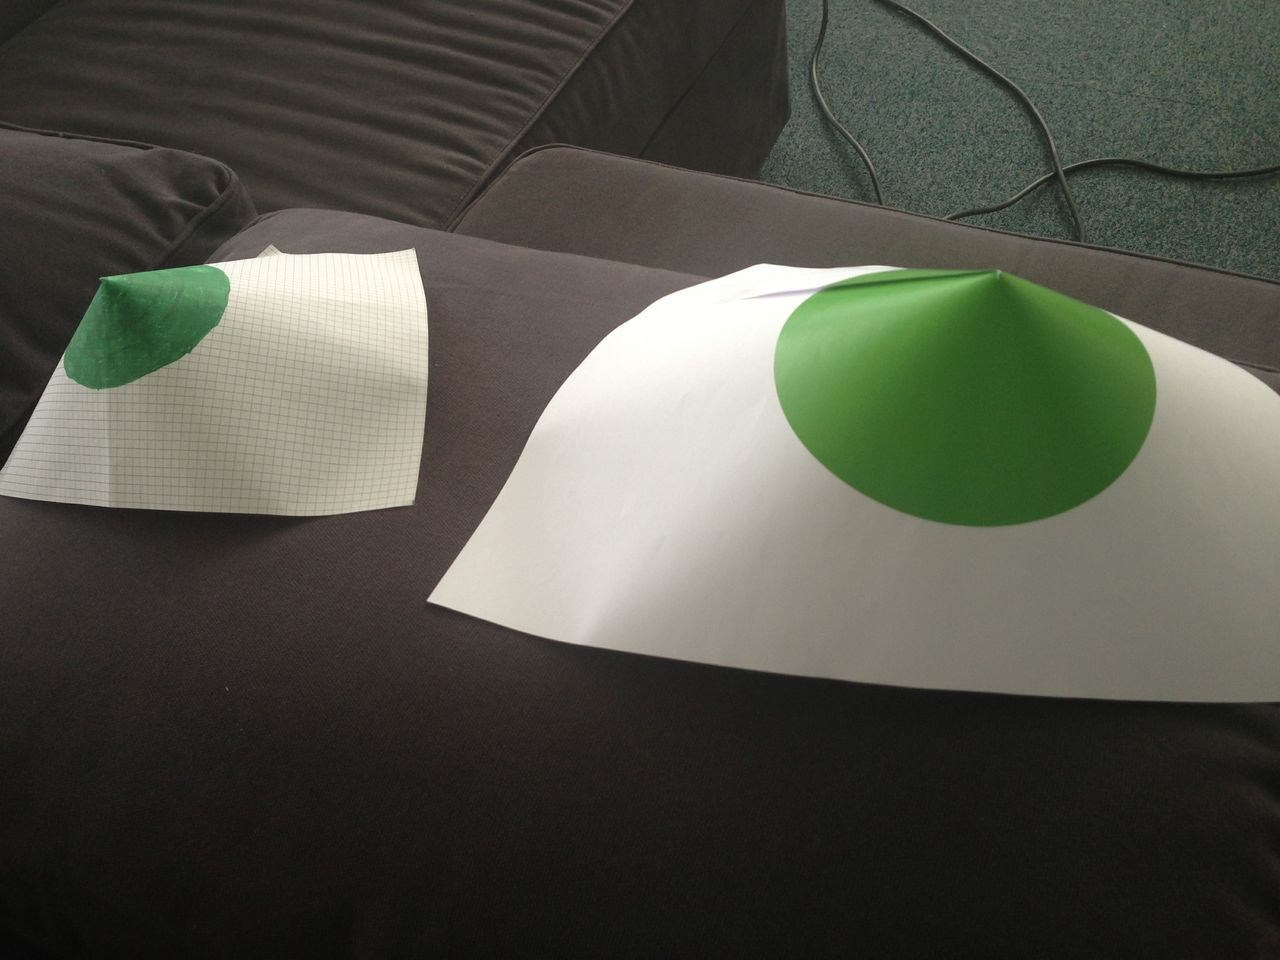
\includegraphics[scale=0.15]{images/small_big_pattern.jpg}
 	\captionof{figure}{Small and big pattern - the big pattern extends the range of the detection}
	\label{fig:small_big_pattern}
\end{center}

\noindent
The algorithm that we describe in this report depends on the pattern that we have chosen. Similarly, it could be adapted in the future to work with different patterns, but we believe that the pattern that we have chosen is easy to build and it provides good results. 
\\\\
The steps for calibration are the following:
\begin{enumerate}
	\item Get the depth map from the Kinect
	\item Get the RGB image from the webcam
	\item Get the RGB image from the Kinect
	\item Perform color filtering on the webcam RGB image
	\item Perform color filtering on the Kinect RGB image
	\item Perform filtering on the depth map based on the Kinect RGB color filtering 
	\item Apply the Gaussian blur on the webcam RGB image and do the difference between two Gaussian blurs
	\item Apply the Gaussian blur on the Kinect RGB image and do the difference between two Gaussian blurs
	\item Pattern detection: Do template matching on the depth image
	\item Pattern detection: Do template matching on the webcam RGB image
	\item Pattern detection: Do template matching on the Kinect RGB image
	\item When all three templates have been matched, we have obtained a set of correspondences
	\item Collect correspondences
	\item Minimization of reprojection error and outlier elimination
	\item Display the Kinect depth map recolored from the webcam RGB image 	
\end{enumerate}

\section{Get the depth map from the Kinect}
\noindent
One of the first steps in any image processing application is to get the images/data that we need for further processing. In our project, the first step is to obtain the depth map provided by the Kinect. Each frame is being captured and stored as an image. Each pixel in the image holds the depth information of that pixel. The depth information can be extracted and we can obtain the depth in millimeters.
\\
For accuracy, the depth map will be stored exactly the way it is received from the Kinect. An example of such an image can be seen below. The completely black pixels show a depth of 0 millimeters. This means that the Kinect cannot obtain any depth information for those pixels. Points that are gray or close to black are the points that are close to the sensor, while points that are far away are white or closer to white. 

\begin{center}
	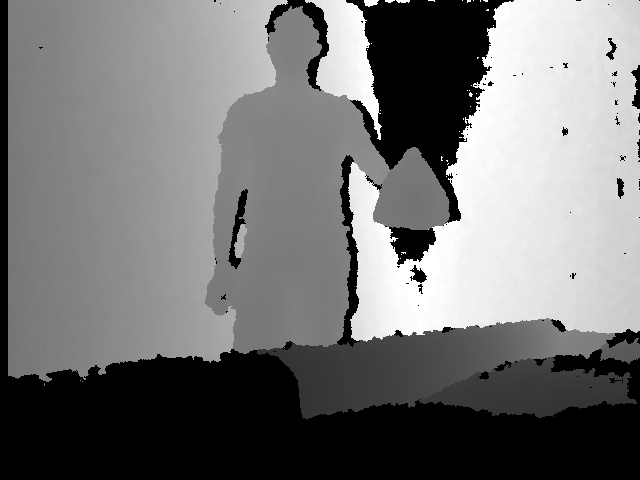
\includegraphics[scale=0.6]{images/original_depth.jpg}
 	\captionof{figure}{Depth image}
	\label{fig:depth_image}
\end{center}

\section{Get the RGB image from the webcam}
\noindent
Once the depth map has been obtained, we must obtain the RGB images from the Kinect and from the normal camera, the webcam. The image from the webcam is also captured frame by frame, it is an image of 640 x 480 pixels. Each point (pixel) stores information about the 3 channels, red, green and blue. 
\\
A sample of the image captured by the webcam can be seen below.

\begin{center}
	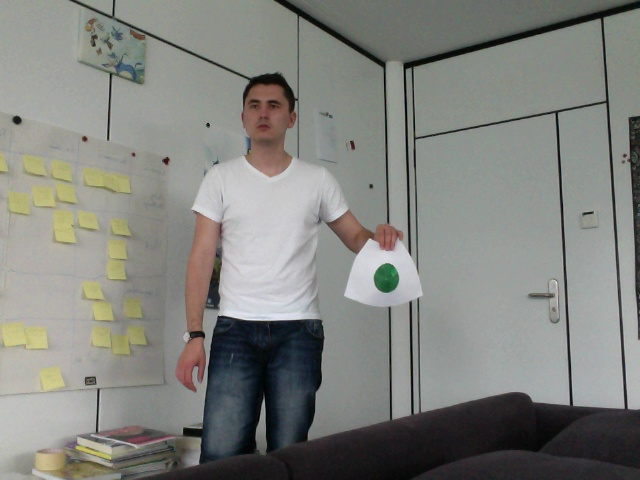
\includegraphics[scale=0.4]{images/rgb_image.jpg}
 	\captionof{figure}{RGB Image}
	\label{fig:rgb_image}
\end{center}

\section{Get the RGB image from the Kinect}
\noindent
Just like in the previous step, we must also get the RGB image from the Kinect's RGB camera. The process is the same as in the previous step, with a small difference that every point (pixel) stores 4 channels (BGRA), not 3 like in the previous case. 
\\ 
A sample of the image can be viewed below. 

\begin{center}
	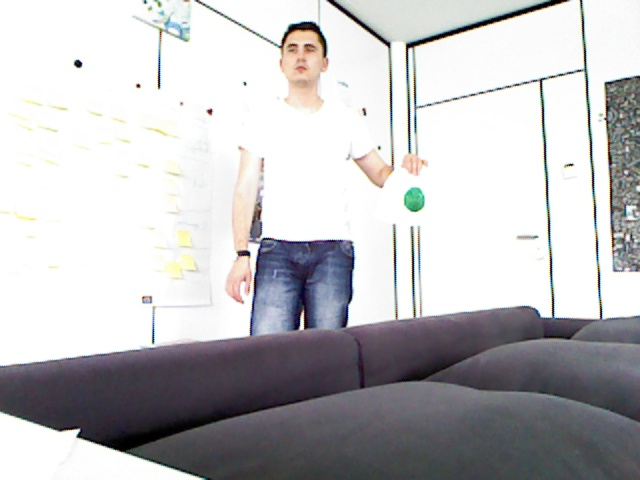
\includegraphics[scale=0.4]{images/kinect_rgb_image.jpg}
 	\captionof{figure}{Kinect RGB Image}
	\label{fig:kinect_rgb_image}
\end{center}

\section{Color filtering on the webcam RGB image}
\noindent
As described in the beginning of this chapter, our goal is to be able to identify a specific pattern. Once the pattern has been detected we can select the center of the pattern and consider a point to which we need to find an equivalent. 
\\
In the sections described below, we will perform template matching on the 3 images that we have obtained previously. Since template matching is not very accurate in all situations, we must find a way in which we can focus our "attention" to only a part of the image and not to the whole image. 
\\
We have identified that performing a color filtering on the RGB images, the result of the template matching (described in the sections below) is greatly improved.
\\
Color filtering is a process in which we filter the RGB image based on a specific color, or a specific range. We know that the tip of our pattern (the cone) is green, so we need to filter out of the image everything that is not green. Once all the points that are not green are filtered from the image, we can try to identify which green area represents the tip of our cone. 
\\
Color separation is quite difficult on the RGB image, so we must first convert the image to the HSV color space. The HSV color space is represented by hue, saturation and value. This allows for a much better segmentation of the image based on the color features. The filtering is easily achieved using the OpenCV function, \emph{cv::inRange}. 
\\
The result of the \emph{inRange} function provided by the OpenCV is a matrix that stores 0 where the color has not been found and 255 where the color of that pixel was in the range specified. Based on this result, we need to compute the center of the color that we have detected. We can do this by computing the median x-axis coordinate and the median y-axis coordinate. This can approximate the position of the peak. Once we have determined the peak we create a window of 100 x 100 pixels which will represent our region of interest. 
\\
An image of the mask can be viewed below.

\begin{center}
	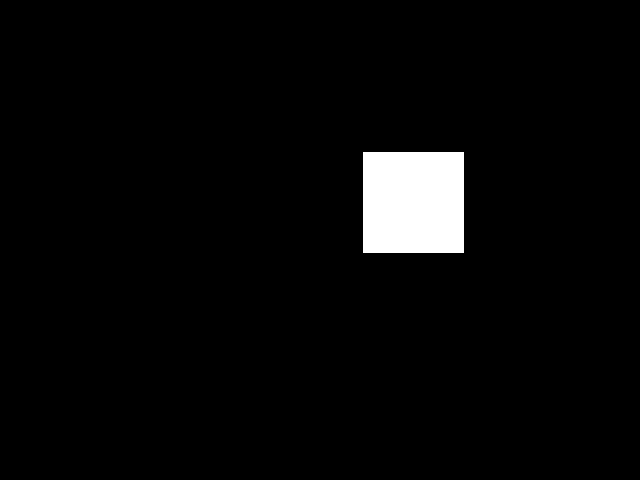
\includegraphics[scale=0.6]{images/color_mask.jpg}
 	\captionof{figure}{Image of a mask}
	\label{fig:color_mask}
\end{center}

\noindent
An image of the RGB image filtered by this mask can be viewed below.

\begin{center}
	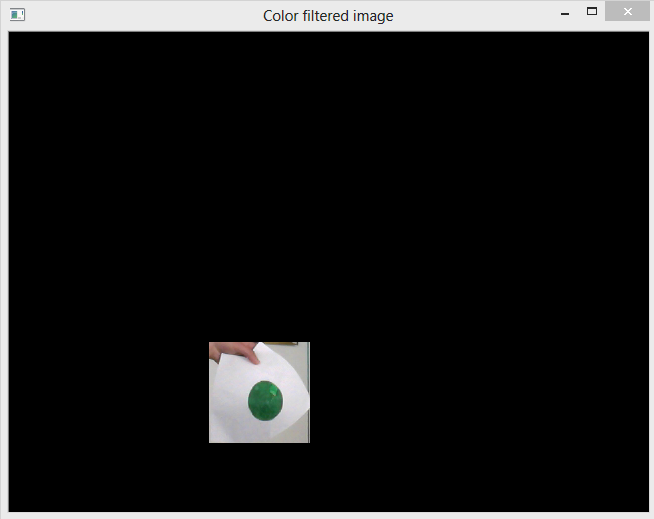
\includegraphics[scale=0.8]{images/color_filtered_image.png}
 	\captionof{figure}{Color filtered image}
	\label{fig:color_filter}
\end{center}

\noindent
As we can observe, the accuracy of the color filtering is very good and the region of interest is exactly what we are looking for. The result of this step will be the input to the next step, where we will apply several times a Gaussian blur on the filtered image. 
\\\\
From an implementation point of view the range of the HSV space for which the color filtering is done is the following

$$ From \; cv::Scalar(38 , 100 , 100) \; To \; cv::Scalar(75 ,255 ,255 ) \; $$

\noindent
The resulting image of this step has the same characteristics as the input image, with the following differences. The resolution is still 640 x 480 pixels, the type of the image is {\bf CV\_8UC3}, but we can only see the image though the window provided by the mask. The rest of the image is black. 

\section{Color filtering on the Kinect RGB image}
\noindent
Color filtering on the Kinect RGB image is done in an almost exact way as the one described previously. The only difference comes from the fact that the Kinect RGB camera is different from the webcam and the color range is also different. 
\\
The range that we have used for the \emph{inRange} function is the following:

$$ From \; cv::Scalar(38 , 110 , 110) \; To \; cv::Scalar(75 ,255 ,255 ) \; $$

\noindent
The resulting image is {\bf CV\_8UC4}, since the input image also stores information on 4 channels. 

\section{Filtering on the depth map}
\noindent
Now that both RGB images have been filtered using a color mask, we also need to filter the depth map. Actually, filtering the depth map is more important than filtering the RGB images. Doing template matching directly on the depth image (each pixel stores the depth in millimeters) can lead to a lot of false positives. The shape of the cone can be easily found in other places, for example the shape of a leg, or a pillow or different objects that can influence the detection. 
\\
Performing a color filtering on the depth map is not really possible since there is no color information. So how can the filtering be achieved? Well, first of all, we have filtered the Kinect's RGB image and we have determined the center of the region of interest. We also know that the Kinect's depth sensor and RGB sensor are calibrated, so we could be able to see which point from the depth image corresponds to the point from the RGB image. 
\\\\
This is quite an easy task to achieve using the SDK provided by Microsoft. We just have to scan the depth map and see each of the depth map's pixel equivalent in the RGB image from the Kinect. The function that does this is 

$$ NuiImageGetColorPixelCoordinatesFromDepthPixelAtResolution $$

\noindent
and it takes as input the resolution of the two images (640 x 480 pixels), a 3D point (current point in the scan through the depth map) and it returns an $X$ and $Y$ coordinate which represent the location of the point we are looking for in the RGB image. 
\\
Once this point has been found, we also apply a mask of 100 x 100 pixels and this way we get our region of interest. 
\\\\
The region of interest after filtering can be seen below:

\begin{center}
	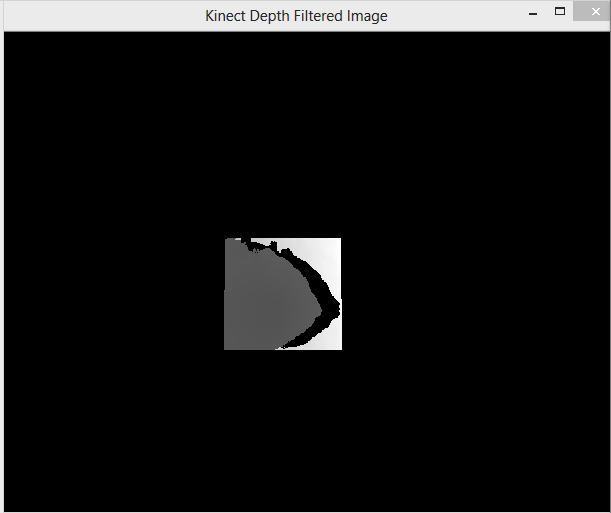
\includegraphics[scale=0.8]{images/depth_filtered_image.png}
 	\captionof{figure}{Depth filtered image}
	\label{fig:depth_filter}
\end{center}

\section{Apply Gaussian blur to the webcam RGB image}
\noindent
Once that we have found the region of interest for our pattern, we need to be able to detect it. The RGB image itself does not provide a lot of information, so we have to further process it. A good way in which we can identify the peak of a cone is to apply a Gaussian blur to the image, applying the Gaussian blur again and then performing the difference between the two images with Gaussian blur. Before applying the Gaussian blur we have to convert the image to gray scale.
\\
The Gaussian blur can be applied using the OpenCV function \emph{cv::GaussianBlur} and we need to specify the input image, the output image and the size of the kernel. 
\\\\
We first apply a Gaussian blur with a kernel size of 21 x 21 pixels. We then apply a Gaussian blur of 21 x 21 pixels. We subtract the two images and we obtain one image where we can observe the peak of the cone. We can notice that it represent a disc like shape with large values, representing a local maximum. Since we have already done color filtering, it is easy to observe that it is the only disc shaped maximum (white disc) in the image, more specifically in the region of interest.
The result of this step can be seen in the image below.

\begin{center}
	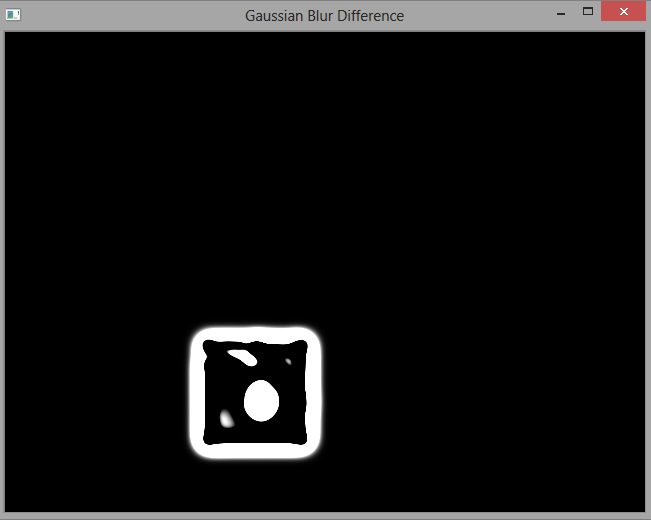
\includegraphics[scale=0.8]{images/gaussian_blur_difference.png}
 	\captionof{figure}{Difference between Gaussian blurs}
	\label{fig:gauss_blur}
\end{center}

\noindent
Another important aspect in this step is obtaining an output image as precise as possible. As a result, we first convert the input images which is {\bf CV\_8UC3} to gray scale and then to {\bf CV\_32FC1}. With floating point values we get much better precision and this will be useful for the next steps where we perform template matching to detect out pattern. 

\section{Apply Gaussian blur to the Kinect RGB image}
\noindent
The process of applying a Gaussian blur to the Kinect RGB image is exactly the same as the one for the RGB image for the webcam. The only difference is the size of the second kernel for the second filtering. It is no longer a 21 x 21 pixels kernel, it is 35 x 35. The value for this kernel has been found empirically. 
\\\\
Just like in the previous case, for greater accuracy, the resulting image will be {\bf CV\_32FC1}.

\section{Pattern detection: template matching on the depth image}
\noindent
Now that all the preprocessing has been done, we can perform template matching to find the pattern that we are looking for. In order to perform template matching we must first select a template. This is done manually and it is read from a file. The size of the template varies between 30 to 60 pixels, depending on the size of the pattern and the range we want to detect it in. 
\\\\
Template matching is done using OpenCV's function \emph{matchTemplate} and it takes as input the depth image, the template for the depth image and the way in which it will evaluate the result. In our project we have chosen {\bf normalized cross-correlation} (\emph{CV\_TM\_CCOEFF\_NORMED}). 

$$ R(x,y) = \frac{\sum\limits_{x',y'} (T'(x',y') \cdot I'(x+x', y+y'))}{\sqrt{\sum\limits_{x',y'} T'(x',y')^2 \cdot \sum\limits_{x',y'} I'(x+x', y+y')^2}}$$

\noindent
This means that in the result of the template matching, the best match will be the point with the maximum value in the image. A value of 1 means a perfect match, while a value of 0 means that the area tested and the template are completely different. 
The template matching will return a point, the left top corner of the match (the template has a square shape). To determine the center of the area where the matching was best we just take the point returned by the template matching function and we add half the size of the width or height of the template. 

$$ depthMatchPoint->x = matchLoc.x + depthTempl.cols/2 $$
$$ depthMatchPoint->y = matchLoc.y + depthTempl.rows/2 $$

\noindent
In order to be sure that the template has been successfully detected we also apply a threshold on the result. Thus, in order to have a valid match, the value returned by the function must be over $0.8$. 
\\\\
Template matching works good, but it is not reliable if the position on the pattern changes in the real world (if the pattern is further away or closer to the camera). When the pattern is far away from the camera, the pattern seems small. To overcome this issue we have used one of OpenCV's functions called \emph{cv::pyrUp} which doubles the width and the height of the initial image. This way, the image is bigger and the pattern is also bigger, so it can be matched with the original template. 

\section{Pattern detection: template matching on the webcam RGB image and Kinect RGB Image}
\noindent
In order to detect the pattern that we have created we also do template matching on the RGB image from the webcam. The template matching process is the same as the one described before. The difference comes from the fact that the template is different. The template is taken from the result of applying to consecutive Gaussian blurs and subtracting them. 
\\
The template matching will return the center point of the template, where the template matches best the current frame. Also the thresholds are different. The template matching on the RGB images are more accurate, so a threshold of $0.75$ is enough to get a good result. 

\section{Validation of template matching}
\noindent
Once the template matching has been performed on the tree images (the depth map, the RGB image from the Kinec and the RGB image from the webcam) we must make sure that the points returned are valid. 
\\
We cannot verify the point from the RGB image of the webcam, but we can check the points provided by the two sensors of the Kinect. This is done using the Kinect calibration. 
\\\\
We use again the function from the Kinect SDK:

$$ NuiImageGetColorPixelCoordinatesFromDepthPixelAtResolution $$

\noindent
and we provide as input the point returned by the depth template matching. The result will be a point $P(x, y)$ which corresponds to a point from the RGB image of the Kinect. We take the point returned from the RGB template matching from the Kinect and we calculate the Euclidean distance between them. If the distance is greater than a certain value (in practice this value is set to 8 pixels), the points are considered to be a bad match. Otherwise we consider the points to be valid and we will feed them to the calibrator. 

\section{Collect correspondences}
\noindent
We now have successfully identified the patterns in all three images and we must calibrate the webcam. 
\\\\
The calibrator has been provided by Julien Pilet, one of the supervisors of this project. The calibration gathers a set of correspondences (a point from the RGB image from the webcam and a point from the depth map) and after enough points have been gathered we try to calibrate the camera. The result of the calibration will be a calibration matrix which can later be used to reproject any point from the depth image to the RGB image. The calibrator tries to minimize the projection matrix A with a Gauss-Newton gradient descent algorithm, by minimizing the sum of the reprojection errors.
\\\\
However, it can happen that the points which have been identified as correct correspondences are actually outliers. A set of points are considered to be outliers if after we reproject the point, the Euclidean distance between the reprojected point and the detected point (from the RGB webcam image) is greater than a certain value. These outliers need to be eliminated because they make the calibration error to be large. 
\\\\
In short, the calibrator is fed with the following points:
\begin{itemize}
	\item depthMatchPoint: P(x,y,z) - a point which has been correctly identified using the template matching technique. The point comes from the depth map of the Kinect.
	\item rgbWebcamMatchPoint: R(x,y) - a point which has been correctly identified using the template matching technique on the RGB image from the webcam. 
\end{itemize}  

\section{Minimization of reprojection error and outlier elimination}
\noindent
As mentioned in the previous case, the first try to calibrate the camera can lead to quite a large error (in practice this error can be between over 20 pixels). This error is large and it will not lead to a good calibration. In order to improve the calibration we must identify which of the points discovered are actually outliers and we need to eliminate them and recalibrate the cameras. 
\\\\
The process of removing the outliers is described below:
\begin{itemize}
	\item Calibrate the camera
	\item Get the projections from the RGB image and the 3d points from the depth image
	\item Reproject all the 3d points
	\item Let's consider P a point from the projections and P' its reprojection using the calibration. If the Euclidean distance between them is larger than a value, we remove this point.
	\item Recalibrate the cameras without the outliers
	\item Repeat the whole process until the reprojection error is minimum.
\end{itemize}

\noindent
What does a minimum reprojection error mean? It can happen that one bad point influences all the other points in the calibration. Taking this into account, we cannot try to remove all the points with a starting error very small. As a result, the iterative calibration considers an error of 1000 pixels. This is a very large value, but it does not change the future outcome. After the outliers which have an error of over 1000 have been eliminated, the error is halved (500 pixels) and the process repeats. The iterative calibration process repeats until we get an error below 2 pixels. 

\section{Depth color reconstruction based on the calibration}
\noindent
Now that we have a calibration and an acceptable error we need a way to visualize the final result of this project. One way to do it is to try to recolor the depth image based on the RGB image from the Kinect. Wihtout a calibration, this process would be impossible since we do not know which points from the depth image correspond to which points from the RGB image of the webcam.
\\\\
With the calibration, we scan the depth map and we reproject each 3D point to get its equivalent from the RGB image. The point from the depth map is colored based on the equivalent point from the webcam's image. 
\\
The result of a depth color reconstruction looks like in the image below.

\begin{center}
	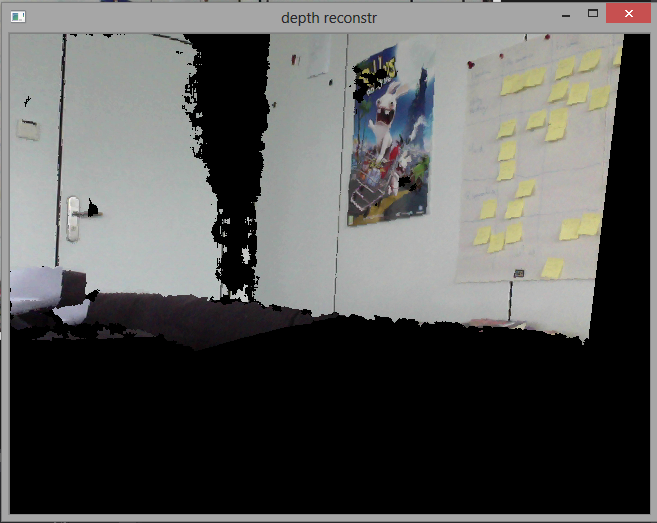
\includegraphics[scale=0.8]{images/depth_reconstruction_1.png}
 	\captionof{figure}{Depth color reconstruction}
	\label{fig:depth_reconstr}
\end{center}   
